\documentclass[conference]{IEEEtran}
\IEEEoverridecommandlockouts

% The preceding line is only needed to identify funding in the first footnote. If that is unneeded, please comment it out.
\usepackage{graphicx}
\usepackage{lipsum}
\usepackage[dvipsnames]{xcolor}
\usepackage{colortbl}
\usepackage{tikz}
\usepackage{pgfplots}
\usepackage{listings,listings-rust}
\usepackage{chronosys}
\usepackage{url}

\pgfplotsset{compat=1.18}
\definecolor{LightCyan}{rgb}{0.88,1,1}

\begin{document}

\title{Ergonomic Systems Programming: Comparing the Developer Experience of Rust and C}

\author{\IEEEauthorblockN{Joshua Ferguson\IEEEauthorrefmark{1}, Stephen A. Torri\IEEEauthorrefmark{2}}
    %\IEEEauthorblockA{
    Department of Computer Science \& Engineering\\ Mississippi State University
    \\
    jmf317@msstate.edu\IEEEauthorrefmark{1}, storri@cse.msstate.edu\IEEEauthorrefmark{2}\\
}

\maketitle

\begin{abstract}
    In systems programming, the choice of programming language significantly impacts developer experience, productivity, and the resulting software quality. Historically, C has been the predominant language in this domain, prized for its performance and resource management capabilities. However, the emergence of Rust presents an intriguing alternative, promising enhanced memory safety and modern language features. This paper aims to rigorously compare the developer experience between Rust and C, focusing on cognitive load, development workflow, and error management.

    Employing a systematic literature review and comparative analysis, we delve into the nuances of systems programming in both languages. Our findings reveal that while Rust imposes a steeper learning curve due to its ownership model and memory safety features, it potentially offers a more robust development experience in the long term, as evidenced by reduced runtime errors and a more expressive type system. In contrast, C's longstanding presence in the field and its direct hardware manipulation capabilities make it a viable choice for specific systems programming tasks.

    The implications of our study are twofold: it guides developers in making informed decisions about language choice based on project requirements and developer expertise, and it contributes to the ongoing discourse on programming language evolution in the context of systems programming. By highlighting the strengths and challenges of each language, this research aims to pave the way for more ergonomic and efficient programming practices in developing critical software systems.
\end{abstract}

\begin{IEEEkeywords}
    Developer experience, DevEx, cognitive load, systems programming, Rust, C
\end{IEEEkeywords}

\section{Introduction}

 {\color{red} The Introduction section of your paper is crucial as it sets the stage for your entire research. Based on the provided excerpt, here are additional suggestions to enhance this section:
  \begin{enumerate}
      \item \textbf{Research Context and Importance}:
            \begin{itemize}
                \item Provide a more detailed context for your research. Discuss the current landscape of systems programming, highlighting the relevance and timeliness of your study.
                \item Emphasize the significance of your research in the broader field. For instance, how does understanding the developer experience in systems programming contribute to the field?
            \end{itemize}

      \item \textbf{Problem Statement}:
            \begin{itemize}
                \item Clearly articulate the problem your research addresses. Why is it essential to compare the developer experience between Rust and C? What gaps in existing literature does your study aim to fill?
                \item Mention any specific challenges or debates in the field that your research speaks to.
            \end{itemize}

      \item \textbf{Research Objectives and Questions}:
            \begin{itemize}
                \item Clearly state the objectives of your research early in the introduction. What do you hope to achieve with this study?
                \item Concisely present your main research questions. This will give readers a clear idea of what to expect in the paper.
            \end{itemize}

      \item \textbf{Background Information}:
            \begin{itemize}
                \item Provide sufficient background on Rust and C, particularly for readers who might not be familiar with these programming languages.
                \item Discuss the historical development and current status of both languages in the context of systems programming.
            \end{itemize}

      \item \textbf{Rationale for Your Approach}:
            \begin{itemize}
                \item Justify the approach you've taken in your research. Why did you choose to focus on these two languages? What makes your comparative analysis methodologically sound?
                \item Discuss any unique perspectives or approaches you bring to this research.
            \end{itemize}

      \item \textbf{Structure of the Paper}:
            \begin{itemize}
                \item Towards the end of the introduction, give a brief overview of the structure of your paper. For example, what will each section cover, and in what order will they appear? This roadmap helps guide the reader through your paper.
            \end{itemize}

      \item \textbf{Thesis Statement}:
            \begin{itemize}
                \item Include a clear thesis statement or a primary claim your paper will support. This should be a concise summary of your main argument or findings.
            \end{itemize}

      \item \textbf{Engagement with Existing Literature}:
            \begin{itemize}
                \item Briefly mention key studies or theories in systems programming that your research builds upon or challenges. This will position your paper within the existing academic conversation.
            \end{itemize}
  \end{enumerate}

  These enhancements will make your introduction more comprehensive, setting a solid foundation for the rest of your paper.}

%  --- Introduction Points --- 
% What was the research topic being investigated?
% Why was this topic important to study?
% What did we know about this topic before I did this study? The reader requires background knowledge to understand the rest of the paper.
% How will this study advance the understanding of computer science?

Systems programming is a somewhat broad area, defined by Encyclopedia Britannica as "the development of computer software that is part of a computer operating system or other control programs "\cite{SystemsProgrammingDefinition}; It's a broad area of software development that includes everything from operating systems to embedded systems, from scientific computing to browsers, just to name a few. However, a few underlying characteristics are common to all of these domains. They all require strict resource management, as they are either resource-constrained or managing resources for applications and services built on top of them. They also tend to be performance-sensitive for much the same reason. They need to be robust and fault-tolerant. Outside of embedded systems, they tend to be generic and usable in as many contexts as possible. Finally, since these are table stakes, they tend to be complex.

The languages we focus on in this literature review are C and Rust. C because, frankly, it's the default in resource constrained or performance focused applications. Rust is a newer language, first developed in 2012, that has been gaining traction in the systems programming space: It's now being used in both the Linux kernel and Windows kernel, and it's employed in 5 of the top 10 fastest web server frameworks. Of the memory safe languages recommended by the NSA, it was the only one that didn't use garbage collection. It's not the only safe contender for the space that still employs C by default, (it would be a disservice to not mention Ada), but

C has been the dominant language for systems programming for decades, and, in some cases, it is still the only viable option. Its support is to some degree universal and functions as a lingua franca for programming languages: most languages have some way to interface with C. Its syntax is simple, and it has a small standard library. Memory management is manual, and while it is statically typed, it is weakly typed. In terms of performance, it's generally considered the gold standard, but it provides none of the abstraction that makes higher-level languages more manageable to use.

Rust's language design centers around compiling time checks to achieve memory safety. It does this through a combination of ownership, lifetimes, and language design itself:
Null values don't exist, all variables are immutable by default, and all errors must be handled explicitly, to give a few examples. To provide a simple example of ownership, consider the following code:
\begin{lstlisting}[language=Rust]
    fn main() {
            let x = vec![1,2,3]
            let y = x;
            println!("{}", x[0])//error 
        }
    \end{lstlisting}
In this example, a vector is created and assigned to the variable x. The value of x is then assigned to y, and thus, y is now the vector owner. Attempting to access the vector from x leads to a compilation error. Lifetimes are a bit more complicated, but the basic idea is that each scope (such as a function or a block) has a lifetime, and the default lifetime of a variable is tied to the lifetime of the content it was created in. This allows the compiler to ensure a variable is not used after its lifetime. To give an example of this, consider the following code:
\begin{lstlisting}[language=Rust]
  fn main() {
      let x;                                       
      {                         
          let y = 5;           

          x = &5; //  error.
      }                    
      println!("{}", x);       
  }                             
   \end{lstlisting}

In this example, the variable's lifetime is tied to its declared scope. When x takes ownership of the reference to y, and then x is used outside of that scope, the compiler generates an error: `y does not live long enough.' If x had not been used, the compiler would have generated a warning (that the value assigned to x is never read) but would have compiled successfully. Lifetimes can be explicitly annotated for instances where you want a reference to outlive the parent scope or need to ensure that a reference is dropped(freed) when and only when the parent scope ends (such as when creating a struct that contains references)

These two concepts are the core of Rust's memory safety and are enforced by static analysis at compile time. Absent the presence of unsafe code(where the developer explicitly tells the compiler that they will handle memory safety) or a bug in the compiler, these features (among others) avoid many of the memory safety issues that plague C (and C++). It's worth noting since we are concerned about its capability as a programming language for domains that are performance critical that on benchmarks, it tends to perform similarly to C and C++\cite{costanzoPerformanceVsProgramming2021}. However, neither performance nor memory safety are the focus of this paper and were only mentioned to provide context.

Developer experience is a broad term with multiple, potentially conflicting definitions. Microsoft, for example, defines developer experience as "How easy or difficult it is for a developer to perform the essential task needed to implement a change "\cite{DeveloperExperienceDevEx} and seems to center its definition around velocity. Interestingly, Github defines it as "how the juxtaposition of developers, processes, and tools positively or negatively affects software development" \cite{davisDeveloperExperienceWhat2023}.

The most comprehensive (or at least measurable) way to define developer experience comes from "DevEx: What Actually Drives Productivity" \cite{nodaDevExWhatActually2023} where it defined the three core dimensions of developer experience as "the ability of the developer to get into a flow state, the length of software feedback loops, and the cognitive load of a given task," and this is the definition we will primarily be using throughout the paper. It's worth noting that many things that can positively or negatively impact these dimensions are organizational and thus out of scope. However, the language and tools used can impact each of these dimensions. For example, feedback loops can be affected by the speed of the compiler, the utility of information provided by static analysis tools(such as the language server), and the ease of integration of telemetry tools (such as profilers and debuggers).

Some things that impact developer experience are unique to the developer and thus unaffected by the language or tools used in "How do you feel developer?" \cite{graziotin2015you}, the authors examined how programmers impacted the ability to execute coding tasks. Affect in this context is not divorced from the development process, as perceptions of tools and problems affect the developer's mood. However, while important to developer experience, these are not considered in this paper. While this is important, it's also challenging to measure and compare, and thus out of scope for this paper.

Development experience is essential to systems programming in that it impacts the ability of developers to reason about the code. Human beings have a finite cognitive capacity influenced by working memory, prior experience, and the current state of mind. The amount of cognitive space allocated to the language or the tooling is nonzero (even in the best case), and as such, finding ways to minimize those costs means more mental resources are focused on the task at hand. It is accessible to missteps when the path is rocky and uncertain, and when the price of a misstep is a disc corruption\cite{larabelItLooksThere2016}, or more famously a rocket explosion\cite{dowsonArianeSoftwareFailure1997}, it is best to keep the path clear.

%  {
%   that both prevent memory safety issues and allow the compiler to make optimizations that would otherwise be impossible (Zero cost abstractions). The language also has a strong focus on ergonomics. To give an example of how the primary tool used with the language (Cargo)
%   is the build system, the package manager, how tests are run, and how documentation is generated -- along with a kitchen sink of other responsibilities. It's also worth noting that it is an expression-based language,
%   which borrows heavily from functional programming, contributing to its learning curve and readability.
%  }{
% It's important to note that Rust also has a concept of soundness, which guarantees that if the code is written in 100\% % safe, Rust cannot have undefined behavior. As such, when looking at studies that compare Rust with C or C++, the community tends to treat
%   violations of soundness as vulnerabilities\cite{xuMemorySafetyChallengeConsidered2021}\cite{traceyGradingCurveHow2023}
%  }

In section \ref{research_method}, we discuss the research objective and criteria that shape the scope of the survey. In section \ref{results}, we discuss the primary research findings that adhere to the rules set in section \ref{research_method}. Finally, in section \ref{results}, we address the research questions set in \ref{research_questions} with drawbacks and future recommendations.

\section{Research Design and Method}
\label{research_method}

{\color{red}In reviewing your Research Design and Method section, here are additional suggestions to enhance its rigor and clarity:
    \begin{itemize}
        \item \textbf{Detailed Explanation of Search Strategy}:
              \begin{itemize}
                  \item Expand on how you developed your search strategy. Explain the rationale behind choosing specific keywords and databases. This explanation will help establish the thoroughness of your literature search.
                  \item If applicable, discuss how you adjusted your search strategy in response to the initial results.
              \end{itemize}

        \item \textbf{Inclusion and Exclusion Criteria}:
              \begin{itemize}
                  \item Provide more detailed explanations for each inclusion and exclusion criterion. For example, explain why you restricted your study to papers published within the last five years.
                  \item Justify your language restriction and discuss how this might limit the scope of your review.
              \end{itemize}

        \item \textbf{Study Selection Process}:
              \begin{itemize}
                  \item Detail the process of screening and selecting studies. For example, did you review titles and abstracts first, followed by full-text screening? Who was involved in this process, and how did you resolve disagreements?
                  \item If applicable, include a flow diagram showing the number of papers identified, screened, eligible, and included in the review (e.g., PRISMA flow diagram).
              \end{itemize}

        \item \textbf{Data Extraction and Synthesis}:
              \begin{itemize}
                  \item Clarify how you extracted data from the selected studies. Mention the type of information you were looking for (e.g., methodologies, findings, context of studies).
                  \item Discuss your approach to synthesizing the extracted data. Did you perform a qualitative thematic analysis, a quantitative meta-analysis, or another method?
              \end{itemize}

        \item \textbf{Quality Assessment of Included Studies}:
              \begin{itemize}
                  \item Add a subsection on how you assessed the quality or credibility of the included studies. This could involve evaluating the study design, methodology, bias, etc.
                  \item Explain how the quality assessment influenced your interpretation of the findings.
              \end{itemize}

        \item \textbf{Addressing Research Bias}:
              \begin{itemize}
                  \item Acknowledge potential biases in your research process, for instance, publication bias, selection bias, or bias in interpreting findings.
                  \item Discuss steps taken to minimize these biases.
              \end{itemize}

        \item \textbf{Reproducibility and Transparency}:
              \begin{itemize}
                  \item Mention any efforts made to ensure the reproducibility of your research. This could include sharing your search strategy, inclusion/exclusion criteria, and data extraction forms.
                  \item If applicable, discuss how others could access the data you used (e.g., through a supplementary file or a data repository).
              \end{itemize}
    \end{itemize}

    Adding these details will strengthen the methodological foundation of your paper, making it more robust and credible for academic scrutiny.}

In the guideline paper by Kitchenham and Charters\cite{GuidelinesPerformingSystematic}, a systematic literature review comprises three steps.

\begin{figure}[ht]
    \centering
    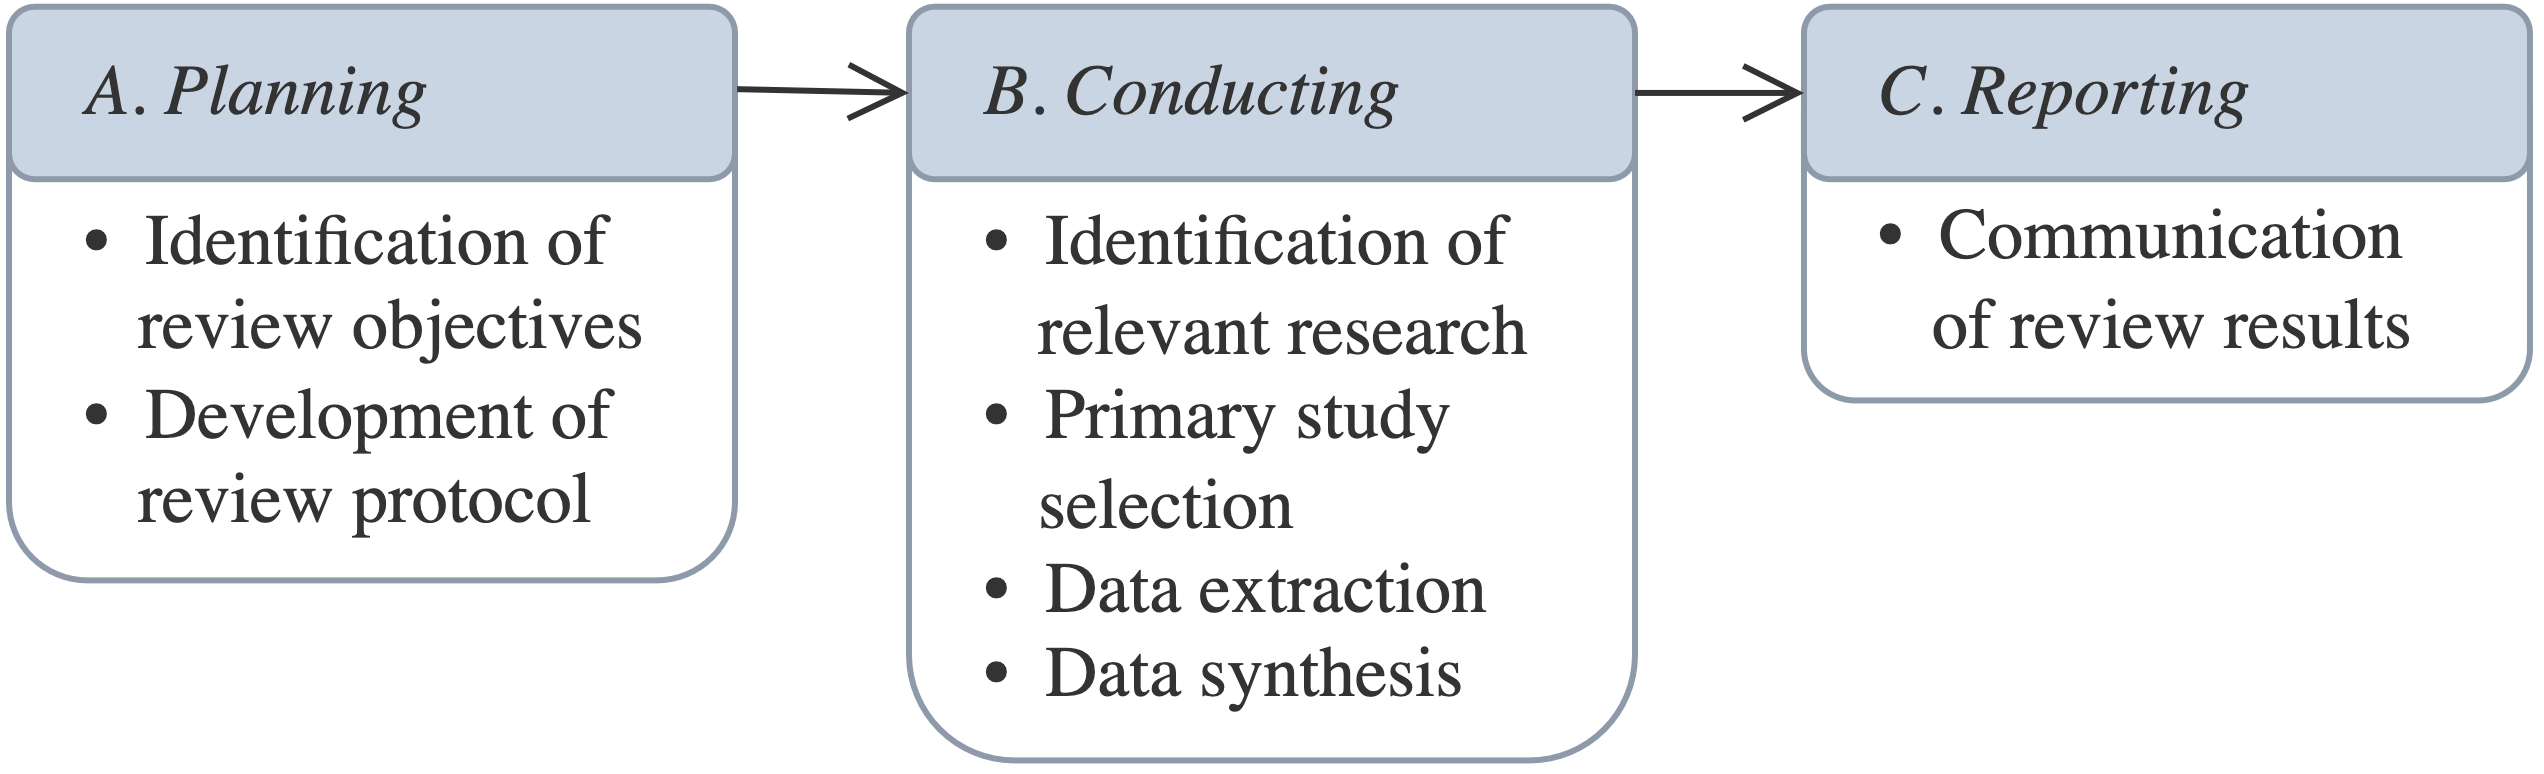
\includegraphics[width=0.489\textwidth]{images/systematic_review_diagram.png}
    \caption{The three phases of a systematic literature review\cite{GuidelinesPerformingSystematic}}
    \label{Fig:slr_diagram}
\end{figure}

\subsection{Planning the review}
\subsubsection{Research questions}
\label{research_questions}

In this sub-section, we aim to address the background, objective, and outcome of conducting the survey.
\begin{itemize}
    \item \textbf{Q1:} {What development friction exist for developers working on systems programming projects, such as the linux kernel}?

          This research question aims to identify the common pain points of developers working on systems programming projects in onboarding and day-to-day development.

    \item \textbf{Q2:} {How does Rust's language design affect the cognitive load of developers in systems programming}?

          This research question looks at how the various attributes of the language, such as the concept of ownership, algebraic data types, and forced error handling, affect the cognitive load of developers, both positively and negatively.

    \item \textbf{Q3:} {How does the workflow (use of tools for common task) differ between the two langauges}?

          This research question will explore how systems programmers accomplish various programming-related tasks, such as debugging, testing, and profiling. We'll look at what tools are used, their strengths and limitations, and the level of integration each device has with the development environment.

          % \item \textbf{Q4:} {What were the motivations behind projects that have done a full or partial migration between the two? How did that affect the developer experience}?\\
          % {In this research question, we'll look at the motivations behind projects that have migrated from C to Rust or have adopted Rust for new development. 
          % We'll also explore the current level of interoperability of the two languages and the outcomes for projects that did a full migration.}
\end{itemize}

\subsubsection{Search Strategy}
\paragraph{\color{Black}Define search terms}{Developer Experience, Cognitive Load, Cyclomatic Complexity, Static Analysis,  Linux kernel, embedded, scientific computing, drivers, browser, network, Rust, C}
\paragraph{\color{Black}Digital libraries used} {IEEE Xplore, ACM Digital Library, Google Scholar, Google}
\paragraph{\color{Black}Any issues using search terms}{
    \begin{itemize}
        \item Developer Experience tends to return papers related to developers' experience level rather than developers' experience.
        \item It doesn't seem easy to find papers at the intersection of systems programming and developer experience
        \item C is a letter, and it seems difficult to limit the results to those related to the programming language if tied to phrases used heavily across domains (such as "cognitive load").
    \end{itemize}
}

\subsubsection{Study selection}
In this sub-section, we aim to define the survey's scope by defining the development areas and the filtering process we followed.

The study selection process is constrained by the inclusion criteria (IC) and exclusion criteria (EC). A paper or source was included if all the following were met:
\begin{itemize}
    \item IC1: The study's target population, or source, were developers working on relevant projects, such as the Linux kernel, or in a domain, such as embedded systems or scientific computing, where highly constrained resource management is a defining characteristic.
    \item IC2: The languages involved in those projects were Rust and C, or the paper discussed topics relevant to developing those languages, such as tooling or ecosystem maturity.
    \item IC3: The paper either focused or touched on the developer experience or related topics such as cognitive load, productivity, or developer velocity
\end{itemize}
A paper will be rejected if any of the following are met:
\begin{itemize}
    \item EC1: The study or source is not in or translatable to English
    \item EC2: If it isn't a paper, the source is neither from a developer working on nor documentation for a relevant project.
    \item EC3: The focus of the source is on performance or memory safety in isolation of all pertinent impact on developers or the development process
\end{itemize}

\subsubsection{\color{Black} Data extraction and systhesis}
\label{data_collection}

As the sources found seem to touch on different intersections of the research questions, we searched for different combinations of search terms relevant to the topics involved. For developer experience, we started with phrases like developer experience, developer velocity, and cognitive load but then moved on to words like "Cyclomatic Complexity" and "Static Analysis."

For systems programming, as it is an umbrella for different categories of projects that are often studied by themselves, we substituted phrases like "embedded," "Linux kernel," and "scientific computing" in a Parenthesized statement in the search engines that supported it. We also searched for the terms "Rust" and "C" in combination with the other words to find papers that discussed the two languages concerning each other.

We filtered papers generally to those published in the last five years, primarily due to lowering the noise of the results(though, unfortunately, some older relevant articles may be filtered out). We tended to cycle between using Google Scholar and then traditional academic databases. While we started primarily with academic databases, the
lack of semantic search tended to increase the number of papers unrelated to programming, and we then transitioned to mainly using Google Scholar, a meta-search engine.

Often, we would find a relevant paper and then look at the documents it cited and the articles that cited it. When searching for non-academic sources, we used Google, and outside of pages that we linked, we only provided definitions for terms used in the paper. We only have one non-academic source, a blog post by one of the primary contributors to Rust's asynchronous programming model.

\subsection{Conducting the review}
\label{conducted_review}

Searching in this manner tended to return a lot of irrelevant results. Developer experience tended to return more results related to the experience level of developers than the experience of development. In a given context, searching for papers associated with C and any other search phrase that wasn't exclusive to programming tended to return primarily irrelevant results. Unless the search engine used had some form of vector search where words are mapped to a vector space, the distance between the vectors determines similarity. We find that papers exploring Rust for some domains related to systems programming generally have some comparison to C and some discussion of the developer experience, but the developer experience is rarely the paper's focus.

We did find one paper(so far) that seems highly relevant to the topic where Rust and C were compared for the difficulty of solving a common HPC benchmarking problem and the relative performance of the two implementations. Papers related to development experience tended to be the most relevant and challenging to find.

\subsubsection{List the number of papers retrieved from digital libraries}

The search was conducted between 2023-09-15 and 2023-11-24; here is the number of papers retrieved from each digital library:
\begin{itemize}
    \item IEEE Xplore: 5
    \item ACM Digital Library: 7
    \item PeerJ: 2
    \item usenix.org: 1
    \item springerLink: 1
    \item Other: 3
    \item Google: 3
    \item Total: 22
\end{itemize}

Other include papers found through Google Scholar but were not hosted on an academic database, such as a thesis, or a paper hosted on a personal website.
Google was for non-academic sources, such as blog posts or GitHub issues.

\begin{table}[!htbp]
    \caption{List of Papers}
    \label{tab:primary_papers}
    \centering
    \def\arraystretch{1.3}
    \begin{tabular}{p{0.1\linewidth}p{0.65\linewidth}p{0.1\linewidth}}
        \hline
        ID  & Author(s)                            & Ref                                                         \\\hline\hline
        S1  & Costanzo, Manuel et al.              & \cite{costanzoPerformanceVsProgramming2021}                 \\\hline
        S2  & Fakhoury, Sarah et al.               & \cite{fakhouryEffectPoorSource2018}                         \\\hline
        S3  & Nadeem, Ayman                        & \cite{nadeemHumancenteredApproachStaticanalysisdriven2022a} \\\hline
        S4  & Davis, Gwen                          & \cite{davisDeveloperExperienceWhat2023}                     \\\hline
        S5  & Noseda, Mario et al.                 & \cite{nosedaRustSecureIoT2022}                              \\\hline
        S6  & Sudwoj, Michal                       & \cite{sudwojRustProgrammingLanguage2020}                    \\\hline
        S7  & Fulton, Kelsey R. et al.             & \cite{fultonBenefitsDrawbacksAdopting2021}                  \\\hline
        S8  & Astrauskas, Vytautas et al.          & \cite{astrauskasHowProgrammersUse2020}                      \\\hline
        S9  & Fagerholm, Fabian et al.             & \cite{fagerholmDeveloperExperienceConcept2012}              \\\hline
        S10 & Graziotin, Daniel et al.             & \cite{graziotin2015you}                                     \\\hline
        S11 & Gulati, Aryan                        & \cite{gulati2022can}                                        \\\hline
        S12 & Hu, Shuang et al.                    & \cite{huComprehensivenessAutomationLifecycle2022}           \\\hline
        S13 & Noda, Abi et al.                     & \cite{nodaDevExWhatActually2023}                            \\\hline
        S14 & Oikawa                               & \cite{oikawaExperienceDevelopingFAT2023}                    \\\hline
        S15 & Developer Experience DevEx           & \cite{DeveloperExperienceDevEx}                             \\\hline
        S16 & Saiorse                              & \cite{saoirseWhyAsyncRust2023}                              \\\hline
        S17 & Xu, Hui                              & \cite{xuMemorySafetyChallengeConsidered2021}                \\\hline
        S18 & Britannica                           & \cite{SystemsProgrammingDefinition}                         \\\hline
        S19 & Guidelines for Performing Systematic & \cite{GuidelinesPerformingSystematic}                       \\\hline
        S20 & Balasubramanian et al.               & \cite{balasubramanianSystemProgrammingRust2017}             \\\hline
        S21 & Rooney, Sean et al.                  & \cite{rooneyEvaluatingFFTPerformance2023}                   \\\hline
        S22 & Tracey, Brendan et al.               & \cite{traceyGradingCurveHow2023}                            \\\hline
        S23 & Nischal, Shrestha                    & \cite{shresthaHereWeGo2020}                                 \\\hline
        S24 & Ardito, Luca et al.                  & \cite{arditoEvaluationRustCode2021}                         \\\hline

    \end{tabular}
\end{table}
\subsection{Threats to validity}

The primary threat to validity is the lack of information related to the development experience of C developers. While we have papers that compare Rust and C in a specific context, such as embedded systems, the focus of those papers is on Rust, and they lack information on the development experience of C developers. We have documents that measure indicators of developer experience, such as the cyclomatic complexity
of a C program, but these approximations only tell us about the complexity of the code. For example, there could exist a tool or idea that makes it easier to reason about the code and is used in professional settings but was not mentioned in the papers selected.

The second threat to validity is selection or publication bias. The papers were selected based on the search terms and their relevance to the research questions. The documents that examined Rust, while critical of the language, tended towards a positive view of the language. It could be that the papers selected are not representative of the general idea of the language or that the documents which are critical of the language were not as discoverable.

The third threat to validity is researcher bias. While we attempted to be as objective as possible since we are familiar with Rust and were not employing a quantitative methodology, our familiarity with the language may have influenced our interpretation of the papers selected.

\section{Results, Discussion, and Implications}
\label{results}

{\color{red}
    Based on the provided suggestions and the content of your "Results, Discussion, and Implications" section, it appears that the following elements might be missing or need further development:
    \begin{enumerate}
        \item\textbf{Detailed Analysis of Results}: While you have presented your findings, analyzing them in more depth is essential. Discuss why these results occurred and how they relate to the existing knowledge in systems programming.
        \item\textbf{Comparative Analysis}: A more explicit comparative analysis between Rust and C could be beneficial. For instance, discuss how specific features of Rust impact developer productivity compared to C, supported by data from your research.
        \item\textbf{Practical Implications}: Expand on the practical implications of your findings. How can developers and teams use this information to make informed decisions about language choice in systems programming?
        \item\textbf{Limitations of the Study}: It's crucial to acknowledge the limitations of your study. Discuss any biases, the scope of literature reviewed, and how these might affect your findings' generalizability.
        \item\textbf{Recommendations for Future Research}: Propose specific areas for future research that arise from your findings. For instance, a more profound exploration into the long-term productivity impacts of using Rust in large-scale systems programming projects.
        \item\textbf{Integration with Research Questions}: Ensure the discussion aligns with your initial research questions. Each key point in your discussion should refer to how it answers or relates to these questions.
        \item\textbf{Concluding Summary}: Conclude the section with a summary that encapsulates the main findings and their significance clearly and concisely.
        \item\textbf{Broader Contextualization}: Discuss how your findings fit into the broader context of programming language evolution, developer experience trends, and the future of systems programming.
    \end{enumerate}

    Incorporating these elements will enhance the depth, clarity, and relevance of your "Results, Discussion, and Implications" section, ensuring that it effectively communicates the significance and impact of your research.}

\subsection{Demographics of the selected studies}
% The demographic subsection provides information about the change in research activity within the scope of the literature survey. This Section should provide the following:
% - Time range of papers in the survey. For example, the articles were published between 2015 and 2023.
% - Activity change that covers the changes in the number of pieces produced. This will require making a list 
%   of documents and their publication date. This helps indicate whether the research area has been gaining attention.

All but 3 Papers selected for this survey were published between 2018 and 2023. two of the outliers were published in 2012\cite{fagerholmDeveloperExperienceConcept2012} and 2015\cite{graziotin2015you} respectively and were included to provide more context on developer experience and how it impacts software development. There was one early paper exploring using Rust in systems programming\cite{balasubramanianSystemProgrammingRust2017} published in 2017.

Not counting the guidelines for performing a systematic literature review\cite{GuidelinesPerformingSystematic}, there were
Seven conference papers, six journal articles, one book entry, four web page/blog posts, and one thesis. Those examining Rust tended to be more recent, with the oldest published in 2020\cite{sudwojRustProgrammingLanguage2020}. The only blog post an individual posted was \cite{saoirseWhyAsyncRust2023}, and was included as it was created by a contributor to the Rust project (and more specifically to the very feature it discussed).

Only a few selected papers were published before 2020, with the oldest being a paper on developer experience published in 2012\cite{fagerholmDeveloperExperienceConcept2012}.
\vspace{3ex}

% six conference papers, six journal articles, one book entry, four web page/blog posts, 1 thesis
\startchronology[startyear=2012,stopyear=2020,height=1pt,  startdate=true, stopdate=true, arrow=false, width=\hsize, box=false]
\chronoevent[date=false]{06/2012}{\cite{fagerholmDeveloperExperienceConcept2012}}
\chronoevent[date=false]{2015}{\cite{graziotin2015you}}
\chronoevent[date=false]{2017}{\cite{balasubramanianSystemProgrammingRust2017}}
\chronoevent[date=false]{05/2018}{\cite{fakhouryEffectPoorSource2018}}
\stopchronology

The majority of the papers were published between 2020 and 2023 inclusively.
\vspace{3ex}

% % Draw the timeline
\startchronology[startyear=2020,stopyear=2024,height=1pt,  startdate=true, stopdate=true, arrow=false, width=\hsize, box=false]
\chronoevent[date=false,markdepth=55pt]{2021}{\cite{fultonBenefitsDrawbacksAdopting2021}}
\chronoevent[date=false,markdepth=55pt]{02/26/2021}{\cite{arditoEvaluationRustCode2021}}
\chronoevent[date=false,markdepth=55pt]{06/2022}{\cite{nosedaRustSecureIoT2022}}

\chronoevent[date=false,markdepth=40pt]{11/13/2020}{\cite{astrauskasHowProgrammersUse2020}}
\chronoevent[date=false,markdepth=40pt]{03/2022}{\cite{nadeemHumancenteredApproachStaticanalysisdriven2022a}}
\chronoevent[date=false,markdepth=40pt]{2023}{\cite{oikawaExperienceDevelopingFAT2023}}
\chronoevent[date=false,markdepth=40pt]{10/2023}{\cite{saoirseWhyAsyncRust2023}}

\chronoevent[date=false,markdepth=25pt]{09/11/2020}{\cite{sudwojRustProgrammingLanguage2020}}
\chronoevent[date=false,markdepth=25pt]{2022}{\cite{gulati2022can}}
\chronoevent[date=false,markdepth=25pt]{2023}{\cite{davisDeveloperExperienceWhat2023}}
\chronoevent[date=false,markdepth=25pt]{03/2023}{\cite{rooneyEvaluatingFFTPerformance2023}}
\chronoevent[date=false,markdepth=25pt]{06/08/2023}{\cite{nodaDevExWhatActually2023}}

\chronoevent[date=false]{06/27/2020}{\cite{shresthaHereWeGo2020}}
\chronoevent[date=false]{09/28/2021}{\cite{xuMemorySafetyChallengeConsidered2021}}
\chronoevent[date=false,]{10/2021}{\cite{costanzoPerformanceVsProgramming2021}}
\chronoevent[date=false]{12/2022}{\cite{huComprehensivenessAutomationLifecycle2022}}
\chronoevent[date=false]{10/2023}{\cite{traceyGradingCurveHow2023}}

% \chronoevent{2023}{\cite{DeveloperExperienceDevEx}}
% \chronoevent{2023}{\cite{SystemsProgrammingDefinition}}
% \chronoevent{2023}{\cite{GuidelinesPerformingSystematic}}

\stopchronology
% \begin{tikzpicture}
%     % Draw horizontal line
%     \node[anchor=west, text width=6cm] at (0,1.1) {Majority of papers published between 2018 and 2023};
%     \draw[align=right, line width=1pt] (0,0) -- (8,0);

%     % Draw vertical lines and labels
%     \foreach \x/\year in {.5/2012, 1.5/2015, 4.5/2018, 8/2023}
%         {
%             \draw (\x,-0.2) -- (\x,0.2);
%             \node[below] at (\x,-0.2) {\year};
%         }

%     % Add labels for the papers
%     \node[anchor=west] at (0,0.5) {\cite{fagerholmDeveloperExperienceConcept2012}};
%     \node[anchor=west] at (1.5,0.5) {\cite{graziotin2015you}};

%     \node[anchor=west] at (7,0.5) {\cite{costanzoPerformanceVsProgramming2021}};
%     \node[anchor=west] at (4.5,0.5) {\cite{fakhouryEffectPoorSource2018}};
%     \node[anchor=west] at (7.5,.5) {\cite{nadeemHumancenteredApproachStaticanalysisdriven2022}};
%     % TODO: Add the rest of the papers
% \end{tikzpicture}

\subsection{Developer Friction in Systems Programming (RQ1)}

This is by far the least covered question currently. Part of the lack of coverage is likely a combination of research focus in systems programming and a limitation of the search terms used. Most results related to C and developer experience, or C projects and developer experience, tended to be related to the experience level of developers, and it was challenging to omit terms related to experience level without omitting relevant results, as the developers contacted during studies are often either students or senior developers.

Another factor was that the papers that compared Rust and C in a specific context (such as embedded systems\cite{nosedaRustSecureIoT2022}) tended to focus more on Rust
and its advantages and disadvantages in that context rather than workflow or tooling used for c development. However, a few things can be derived despite the lack of emphasis on C.

First, in the paper on Rust in embedded systems\cite{nosedaRustSecureIoT2022}, the authors talked about the utility of user-defined types in ensuring the correct order of initialization of the GPIO output pin and the UART driver. In their words, "Encoding the pin state like this ensures that misconfiguration (or simply forgetting to initialize) is an issue of the past." There is a stringent requirement to ensure correctness, and it requires a degree of understanding of the underlying physical system.

C's manual memory management and weak typing can benefit embedded systems, allowing for more direct control over the hardware. However, this sets the bar for entry higher, putting the requirement for ensuring correctness solely on the developer. In that same paper, the authors also mentioned using a static analysis tool for C, the type of memory bugs they can detect, and their limitations. Static analysis tools work well so long as the source code being analyzed is available, which is not the case for dependencies.

The research compares the likelihood of new contributors introducing bugs on their first contribution in Rust and C++ in the Mozilla project, where the Rust code replaced C++ code. Thus, a direct comparison could be made.\cite{traceyGradingCurveHow2023}. In this paper, the authors discuss the difficulty in attracting new contributors to existing projects and how efforts to do so by Mozilla's open-source initiatives often stir anxiety in existing maintainers. The first-time contributors are often inexperienced, and existing maintainers don't have the infrastructure to support them. Often, they introduce bugs, and most don't contribute again.

Lastly, due to manual memory management and lack of abstraction, it isn't easy to use a language like C in domains like HPC and scientific computing to create software that is both scalable and maintainable\cite{costanzoPerformanceVsProgramming2021}.

% Touched on by secure IOT, maybe can rust replace c and the HPC paper

\subsection{How does Rust's language design affect the cognitive load of developers in systems programming? (RQ2)}

In \cite{fultonBenefitsDrawbacksAdopting2021}, most of the
participants in the survey found Rust more challenging to learn than other languages. The concept users struggled with the most when initially learning Rust was ownership, which is unsurprising given the relative novelty of ownership in programming languages. In \cite{shresthaHereWeGo2020}, the authors discussed the factors that make new programming languages more challenging to learn and two of the factors where participants mentioned Rust explicitly is when the language concept either requires a mind-shift or doesn't map to something they already know. Other things contributing to the initial learning curve are that it is expression-based and borrows heavily from functional programming.
% Also, speaking from experience, certain patterns are common in object-oriented programming that new developers tend to try to use in Rust, like grouping data together 

% {
%     There is a tradeoff in Rust between the initial learning curve and the cognitive load of practiced Rust developers.   The learning curve is also impacted by the fact that Rust explicitly
% doesn't use inheritance and (speaking from experience) the tendency to try to use object-oriented programming patterns
%, such as wrapping all data in a struct makes for a difficult transition. In that example, the reason is that if you have a
%     function where only some data needs to be mutable, you have to either make the entire struct mutable(which means borrowing it exclusively) or
%     use interior mutability, which can quickly become a complicated endeavor.
% }

The tradeoff is that once you've learned the language and have reached the point where you're comfortable with it, the guarantees provided by the language and the compiler make it easier to reason about the code and provide a degree of confidence that the code will behave as expected. This is partly due to the ability to use the type system to enforce invariants, which moves what would otherwise be runtime errors to compile time errors\cite{nosedaRustSecureIoT2022}.

In \cite{balasubramanianSystemProgrammingRust2017}, the author brings up the utility of Rust's properties (which he incorrectly describes as a linear type system rather than affine) and uses this to implement a Software Fault Isolation (SFI) system and argues that Rust enables SFI with lower overhead than "any mainstream language." The premise is that since each component only has access to objects granted to it by the allocator or other members, it could be implemented without copying.

This does seem to affect how much users trust their code. In \cite{fultonBenefitsDrawbacksAdopting2021}, 90\% of the interview participants slightly or strongly agreed with the sentiment that their production code was bug-free. While there was a small sample size for the interview portion, and the participants were self-selected, that degree of trust seems to be backed up by the data. In\cite{xuMemorySafetyChallengeConsidered2021}, all 186 memory safety bugs examined required unsafe code. Many of the CVEs were mild soundness issues that open the possibility of undefined behavior in safe Rust.

A quick note about soundness: Rust has a concept of soundness, which guarantees that if the code is written 100\% safe, Rust cannot have undefined behavior. To say that a library or application is sound means that all possible uses cannot lead to undefined behavior. The program will execute in a predictable, deterministic manner. These are guarantees that the community takes seriously, and often, violations of soundness are (arguably misguidedly) reported and treated as vulnerabilities\cite{xuMemorySafetyChallengeConsidered2021}\cite{traceyGradingCurveHow2023}.
These vulnerabilities would not exist in C or C++ simply because they make no such guarantees.

When comparing the likelihood of new contributors introducing vulnerabilities in Rust and C++ in the Mozilla project, the author found that first-time Rust contributors were 70 times less likely to introduce a vulnerability. Many of the vulnerabilities in the Rust code were soundness issues, and all required unsafe code\cite{traceyGradingCurveHow2023}. It's worth noting that, as a few people in the CPP subreddit pointed out, the comparison was not entirely fair, and the multiple of 70 is likely an overestimate. On the first point, the rust code was replacing C++ code; thus, some of the contributors likely referenced the module they
were replacing. On the second point, looking at the data on commits and vulnerabilities listed in the study leads to a much more conservative interpretation (5x or 6.5x).

%TODO: add a paragraph for how users are using unsafe

As far as the inherent complexity of the language, Rust seems to sit between C, C++, and higher languages. In \cite{arditoEvaluationRustCode2021}, Rust was compared to a set of other languages (including C) in terms of cyclomatic complexity, Halstead metrics, cognitive complexity, and Maintainability Index. These metrics are all related to the cognitive load of developers.

Cyclomatic complexity measures the number of linearly independent paths through a program and estimates how difficult it is to test and modify. Halstead metrics are a set of metrics that approximate software properties such as the length(the number of operators and operands), volume(information content of a program), and time it would take a programmer to implement, to name a few.

Cognitive complexity measures how difficult it is to understand a piece of code intuitively and is based on the sum of the cognitive weights of basic software control structures. The maintainability index is a composite metric that attempts to approximate the maintainability of a piece of software. In all the metrics, Rust outperformed C (and C++), though it's worth mentioning that it performed worse than higher-level languages in all except cognitive complexity. It had the lowest cognitive complexity of all the languages tested.

In\cite{nodaDevExWhatActually2023}, the authors stated that one of the primary factors in developer experience is the length of feedback loops. One of the areas that Rust is lacking is compile time, and for larger projects, especially those that use macros, generics, and user-defined types, compile times can be a significant issue. Part of the issue is that the Rust compiler frontend is single-threaded, though there is work being done to address this \cite{TrackingIssueParallel}.

\subsection{Differences in Workflow (RQ3)}

%in Rust, heavy use of static analysis, and Cargo as the goto tool for everything
To a certain extent, this, like the findings for RQ1, is difficult to answer for C without drawing on personal experience. The papers that compared the two languages mentioned tools and workflow information for C in passing. In \cite{nosedaRustSecureIoT2022}, the authors mentioned a series of static analysis tools for C and what type of (memory safety) issues they could be used to detect. In \cite{costanzoPerformanceVsProgramming2021}, the authors briefly laid out the C implementation, its use of OpenMP, and the directives used for things like SIMD operation. In \cite{saoirseWhyAsyncRust2023}, the author talked about how userspace
concurrency is handled in C: "People implementing highly performant network services in languages without facilities for user-space concurrency like C tend to implement them using a hand-written state machine."

Given the (current) lack of information on the workflow for C, I can only make broad assumptions about the general development process in C. First, since there is no package manager, a few large libraries are used almost universally for some tasks, such as openMP. Most things are implemented from scratch as needed.
Static analysis tools exist but play a minor role in the development process. Third, writing code is more accessible, but it requires more is left to the developer to ensure correctness. Lastly, there are tools for most tasks, but developers (or teams) are partially rolling out their tooling.

In Rust, there is more of a focus on code reuse due to Cargo's function as a package manager and tool for publishing packages (called crates). There are currently 132,254 published crates, and while a large portion of those are either small utilities or are no longer maintained, there is a crate for most tasks. Because Cargo is also how you generate documentation and publication automatically generates documentation from the public API, documentation is current and in at least a basic form for all crates. Each crate links to a repository, and an entry on doc.rs, which is a site that hosts documentation for crates, it also contains the source for that specific published version of the crate.

%in Rust heavy use of static analysis, and Cargo as the goto tool for everything
Static analysis is built into the compiler; it is how ownership and lifetimes are enforced, and violations of those rules can be detected without compiling via Cargo clippy, which the language server rust-analyzer can call. This makes compilation less prominent in the development process.

% \subsection{Motivations for Migration(RQ4)}
% {\color{OrangeRed} \lipsum[1-2]}

\section{Conclusion}
 {\color{red}Based on the conclusion you provided and the essential elements of a strong conclusion, here are specific aspects that appear to be missing or could be enhanced:
  \begin{enumerate}
      \item\textbf{Direct Connection to Research Questions and Objectives}: Your conclusion should explicitly revisit the research questions and objectives stated at the beginning of your paper. This would help readers see how your findings have addressed these questions.
      \item\textbf{Detailed Implications for Practice}: While you mention the impact of your findings, specific implications for practitioners in systems programming are not clearly articulated. Detail how developers or teams can apply your results in real-world scenarios.
      \item\textbf{Explicit Statement of Limitations}: There's a lack of a clear statement on the limitations of your study. This could include methodological constraints, the scope of literature reviewed, or potential biases. Discussing rules adds credibility to your research.
      \item\textbf{Focused Recommendations for Future Research}: Your conclusion could benefit from more specific suggestions for future research. Identify particular gaps your study has revealed and suggest potential areas or methodologies for further investigation.
      \item\textbf{Final Synthesis}: A final synthesis that ties together your key findings, their implications, and the future outlook of the field would provide a strong closing statement. This should encapsulate the essence of your research compellingly and memorably.
      \item\textbf{Reflective Insight}: The conclusion could be enriched with reflective insights about what your research reveals about the evolution of systems programming or the broader trends in programming languages.
      \item\textbf{Closing Remark}: Conclude with a strong, impactful statement that emphasizes the significance of your research, ideally leaving the reader with a sense of the study's broader importance and potential impact in the field.
  \end{enumerate}
  Incorporating these elements will make your conclusion more robust and ensure it effectively captures the essence and impact of your research.}
There are areas where Rust is lacking: its ecosystem varies in maturity, and its compile times can be terrible under the right circumstances. It's hard to learn if you compare it to C, C++, or anything else that isn't Haskell. However, it's also a language designed to be challenging to use incorrectly and one that, by some metrics, is relatively easy to reason about. It's a language that, once learned, provides an ergonomic set of tradeoffs that helps developers write correct and performant code.

There is an inherent difficulty in the tasks relevant to the domain: writing device drivers, managing an OS, or writing a browser that connects and protects users from the internet. C has been the go-to language for these tasks for decades; unfortunately, that is unlikely to change (soon). It's fast, and in experienced hands, its memory safety issues can be mitigated, but if all it took to write correct code were experience, we wouldn't have the bugs we have today.

Perhaps an illustrative example might be useful in understanding the importance of developer experience to systems programming. In  \cite{rooneyEvaluatingFFTPerformance2023}, the author was comparing the performance of RustFFT and FFTW(written in C), two libraries for performing Fast Fourier Transforms, an algorithm that plays an important role in signal processing and often AI. The RustFFT consistently beat FFTW in the benchmarks, and it was designed that the behavior of the library and it's output matched FFTW. If we are willing to put aside the possibility that the developer of RustFFT was a better developer or that rust was inherently faster (both of which are arguably false), if rust offered a better developer experience, this meant faster development iterations when utilizing new instruction sets, fewer bugs, and an easier time managing the complexity that comes with writing a cross-architecture library that uses a planner to perform FFTs as fast as the hardware will allow without making a custom FFT specific to that hardware.

In some ways, this isn't a fair comparison. Rust was built to address developers' issues and frustrations with C++, which itself had an origin not too different in it's relation to C. I strongly suspect that the community is so focused on defacto standards and one single build tool that does most things because of how fragmented the C++ ecosystem is. Drawing on personal experience, it has some of the best error messages out of any language I've used, and the level of integration between the language and the tooling means I spend less time on the meta tasks of development, such as configuring my editor or build system, and more time on the actual task at hand.

One of the things mentioned in \cite{traceyGradingCurveHow2023} is how the risk of introducing vulnerabilities limits open-source projects' ability to attract and support new contributors. Rust provides a way to mitigate that risk and leverage the type of system to communicate and enforce relationships between components. At the very least, there is a victory in knowing that the PR you just merged from some well-intentioned stranger of questionable competence won't cause an explosion.

\subsection{Future Work}

I had a few questions not addressed in the papers I found. The First is how Rust compares to c (and c++) when using \texttt{\#![no\_std]}, which is a crate attribute that causes the compiler to not link to the standard library. It is used in embedded systems or when limited space is available. I'm curious how the lack of a standard library affects development.

Second, if there is some measure of information density per line or expression, how would Rust compare to other languages? I'm curious how much information is conveyed per line of code between the type system, lifetime annotation, and explicit mutability. The third is for programs with variants in Rust and C; how complex is the implementation? This, again, draws perhaps too much from personal observation. Still, I've noticed a tendency of rust developers to do things like attempt to eliminate clones (method for deep copying),
among other attempts to reduce the amount of memory allocated. I'm curious whether this `tendency' is expected and how much of an impact it has on the complexity of
a rust program compared to its C counterpart.

\bibliographystyle{IEEEtran}
\bibliography{references}

\end{document}
